% =====================================================================
%  1bat-ud6-7.tex  —  SESSIÓ 7: Diagrames d'arbre: estructurar les rutes
%  (sense preàmbul: s'inclou des de main.tex)
% =====================================================================
\horatitol{Sessió 7 — Diagrames d'arbre: estructurar les rutes}%
{Quan un procés té diverses etapes encadenades, el diagrama d'arbre les ordena: multipliquem al llarg d'un camí i sumem les rutes que porten al mateix lloc.}

\subsection{Idea clau}

Amb les condicionades mecanitzades (sessions 5 i 6), aprenem ara l'eina visual central
de l'Activitat 1: el \textbf{diagrama d'arbre}. Serveix per estructurar processos amb
\textbf{diverses etapes encadenades} (per exemple, les fases d'un programa social) i
calcular-ne les probabilitats de manera ordenada.

\begin{idea}
\textbf{Com es construeix i es recorre un arbre}
\begin{itemize}[leftmargin=1.4em, itemsep=2pt]
  \item Cada \textbf{branca} representa un resultat possible amb la seva probabilitat.
  \item Les branques que surten d'un \textbf{mateix punt} han de \textbf{sumar $1$}.
  \item \textbf{Multiplicar} les probabilitats al llarg d'un camí dóna la probabilitat
        d'aquella \textbf{ruta completa}.
  \item \textbf{Sumar} les rutes que porten a un mateix resultat dóna la seva
        \textbf{probabilitat total}.
\end{itemize}
\textbf{Connexió:} les branques de la segona etapa són, de fet, probabilitats
\textbf{condicionades} (depenen del que ha passat a la primera).
\end{idea}

\subsection{Exemples}

\begin{exemple}[un arbre de dues etapes]
Triem una de dues bosses i, després, en traiem una bola. La \textbf{bossa 1} ($P=0,4$)
té un $70\%$ de boles vermelles; la \textbf{bossa 2} ($P=0,6$), un $50\%$. L'arbre:

\begin{center}
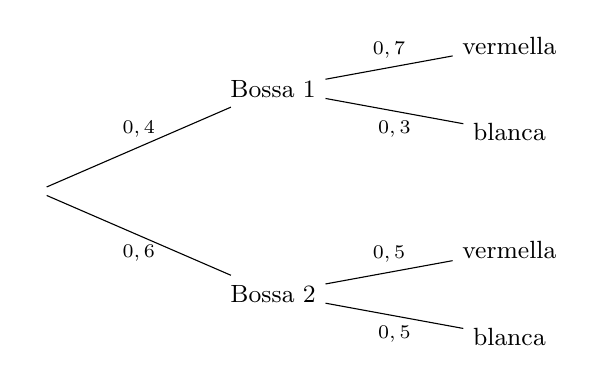
\begin{tikzpicture}[level distance=30mm, sibling distance=9mm,
   every node/.style={font=\small}, grow=right,
   level 1/.style={sibling distance=26mm},
   level 2/.style={sibling distance=11mm}]
\node {} 
  child {node {Bossa 2}
    child {node {blanca}     edge from parent node[below,font=\scriptsize]{$0,5$}}
    child {node {vermella}   edge from parent node[above,font=\scriptsize]{$0,5$}}
    edge from parent node[below,font=\scriptsize]{$0,6$}}
  child {node {Bossa 1}
    child {node {blanca}     edge from parent node[below,font=\scriptsize]{$0,3$}}
    child {node {vermella}   edge from parent node[above,font=\scriptsize]{$0,7$}}
    edge from parent node[above,font=\scriptsize]{$0,4$}};
\end{tikzpicture}

\figcap{Cada parell de branques suma $1$ ($0,4+0,6$; $0,7+0,3$; $0,5+0,5$).}
\end{center}

\noindent\textbf{Probabilitat de treure vermella} (sumant les dues rutes que hi porten):
\[
P(\text{vermella})=\underbrace{0,4\per 0,7}_{\text{bossa 1}}+\underbrace{0,6\per 0,5}_{\text{bossa 2}}
=0,28+0,30=0,58.
\]
\end{exemple}

\begin{exemple}[llegir totes les rutes]
El mateix arbre té \textbf{quatre} rutes completes (multiplicant al llarg de cada camí):
\[
\begin{aligned}
&\text{bossa 1 i vermella: } 0,4\per 0,7=0,28, &\quad &\text{bossa 1 i blanca: } 0,4\per 0,3=0,12,\\
&\text{bossa 2 i vermella: } 0,6\per 0,5=0,30, &\quad &\text{bossa 2 i blanca: } 0,6\per 0,5=0,30.
\end{aligned}
\]
\textbf{Comprovació:} totes les rutes sumen $0,28+0,12+0,30+0,30=1$, com ha de ser.
\end{exemple}

\subsection{Exercicis resolts}

\begin{exresolt}[recórrer un arbre donat]
Un procés té dues etapes. A la primera, $A$ passa amb $P=0,3$ i no passa amb $P=0,7$.
Si $A$ passa, a la segona etapa $B$ passa amb $P=0,8$; si $A$ no passa, $B$ passa amb
$P=0,2$. Calcula la probabilitat que $B$ acabi passant.
\solucio
Hi ha dues rutes que porten a $B$:
\[
\begin{aligned}
\text{($A$ i després $B$): } &0,3\per 0,8=0,24,\\
\text{(no $A$ i després $B$): } &0,7\per 0,2=0,14.
\end{aligned}
\]
Sumant les dues rutes:
\[
P(B)=0,24+0,14=0,38.
\]
\resposta{$P(B)=0,38$.}
\end{exresolt}

\begin{exresolt}[una ruta concreta]
Amb el mateix arbre, quina és la probabilitat que $A$ \textbf{i} $B$ passin tots dos?
\solucio
És una sola ruta (la del camí $A\rightarrow B$), de manera que multipliquem:
\[
P(A\cap B)=0,3\per 0,8=0,24.
\]
\resposta{$P(A\cap B)=0,24$.}
\end{exresolt}

\subsection{Exercicis per fer}

\begin{exercicis}
\begin{exlist}
  \item En un arbre, d'un node surten dues branques amb probabilitats $0,65$ i una
        altra desconeguda. Quant val la branca que falta? Per què?
  \item Un procés té dues etapes. A la primera, $A$ passa amb $P=0,5$. Si $A$ passa, $B$
        passa amb $P=0,6$; si no, $B$ passa amb $P=0,2$. Dibuixa l'arbre i calcula
        $P(B)$.
  \item Amb l'arbre de l'exercici 2, calcula la probabilitat de la ruta «$A$ i $B$» i la
        ruta «no $A$ i $B$».
  \item Una urna té $P(\text{vermella})=0,4$. Es fan dues extraccions \textbf{amb
        reposició} (es torna la bola). Dibuixa l'arbre de dues etapes i calcula la
        probabilitat de treure \textbf{dues vermelles}.
  \item \textbf{(Compte)} Un company, per calcular la probabilitat d'un resultat al qual
        porten \textbf{dues} rutes, multiplica les dues rutes en comptes de sumar-les.
        Quin error comet? Quan es multiplica i quan se suma?
  \item \textbf{(Raonament)} Per què les branques que surten d'un mateix punt han de
        sumar $1$? Què voldria dir que en sumessin $1,2$?
\end{exlist}
\end{exercicis}

% ---------------------------------------------------------------------
\fullsolucions{Sessió 7}
\begin{solucions}
\begin{sollist}
  \item La branca que falta val $1-0,65=0,35$, perquè les branques d'un mateix node han
        de sumar $1$ (algun dels resultats ha de passar).
  \item Rutes cap a $B$: $0,5\per 0,6=0,3$ i $0,5\per 0,2=0,1$.
        $P(B)=0,3+0,1=0,4$.
  \item Ruta «$A$ i $B$»: $0,5\per 0,6=0,3$. Ruta «no $A$ i $B$»: $0,5\per 0,2=0,1$.
  \item Amb reposició, cada extracció té $P(\text{vermella})=0,4$ (independents). Dues
        vermelles: $0,4\per 0,4=0,16$.
  \item Comet l'error de \textbf{multiplicar quan havia de sumar}. Es \textbf{multiplica}
        al llarg d'\emph{una} ruta (per encadenar etapes); se \textbf{suma} quan
        diferents rutes porten al \emph{mateix} resultat final.
  \item Perquè, d'un mateix punt, \textbf{algun} dels resultats possibles ha de passar
        amb seguretat: la suma de totes les opcions és el succés segur, que val $1$. Que
        sumessin $1,2$ voldria dir que hi ha un error (probabilitats mal posades), perquè
        la probabilitat total no pot superar $1$.
\end{sollist}
\end{solucions}
